\section{Grundlagen des Protokolls}
\label{sec:grundlagen_des_protokolls}


Um die Peer-to-Peer Funktionalität für das Protokoll dieser Arbeit zu gewährleisten, wird ein mehrschichtiges Verfahren verwendet.

Für den effizienten Aufbau einer Direktverbindung zwischen zwei Teilnehmern kamen Chord und Kademlia in die engere Auswahl, welche beide lange Gegenstand intensiver Forschung waren, sowohl in der Industrie als auch in der akademischen Welt \parencite[S. 808]{MedranoChavez_ChordKademliaHighChurnScenarios}. 
Das Chord-Protokoll und das Kademlia-Protokoll sind zwei grundlegend verschiedene Ansätze zur Organisation von Peer-to-Peer-Netzwerken. Beide Protokolle sind strukturiert und bieten eine effiziente Ressourcenlokalisierung, aber sie unterscheiden sich in ihrer Routing-Struktur und der Art und Weise, wie sie die Knoteninformationen verwalten.

\subsubsection{Chord}
Chord basiert auf einer Ringstruktur (siehe Abbildung \ref{chord_ring}), bei der die Knoten in einem Ring angeordnet sind und jeder Knoten für einen bestimmten Schlüsselbereich verantwortlich ist. Die Verbindungen zwischen den Knoten sind durch ihren Platz im Ring definiert, wobei jeder Knoten eine Verbindung zu seinem nächsten Nachbarn im Uhrzeigersinn hat. Ein Knoten besitzt zwei Informationsmengen: eine \textit{Successor-Liste} und eine \textit{Finger-Tabelle}. Die Successor-Liste enthält die Knoten, die direkt nach dem Knoten im Uhrzeigersinn im Ring kommen. Die Anzahl der dort enthaltenen Knoten hängt davon ab, wie viele Knoten im Netzwerk insgesamt vorhanden sind. Die Finger-Tabelle enthält die Knoten, die für die Schlüsselbereiche verantwortlich sind, die durch eine Berechnung auf der ID des Knotens basieren \Parencite[S. 810-811]{MedranoChavez_ChordKademliaHighChurnScenarios}.

\begin{center}
    \captionsetup{type=figure}
    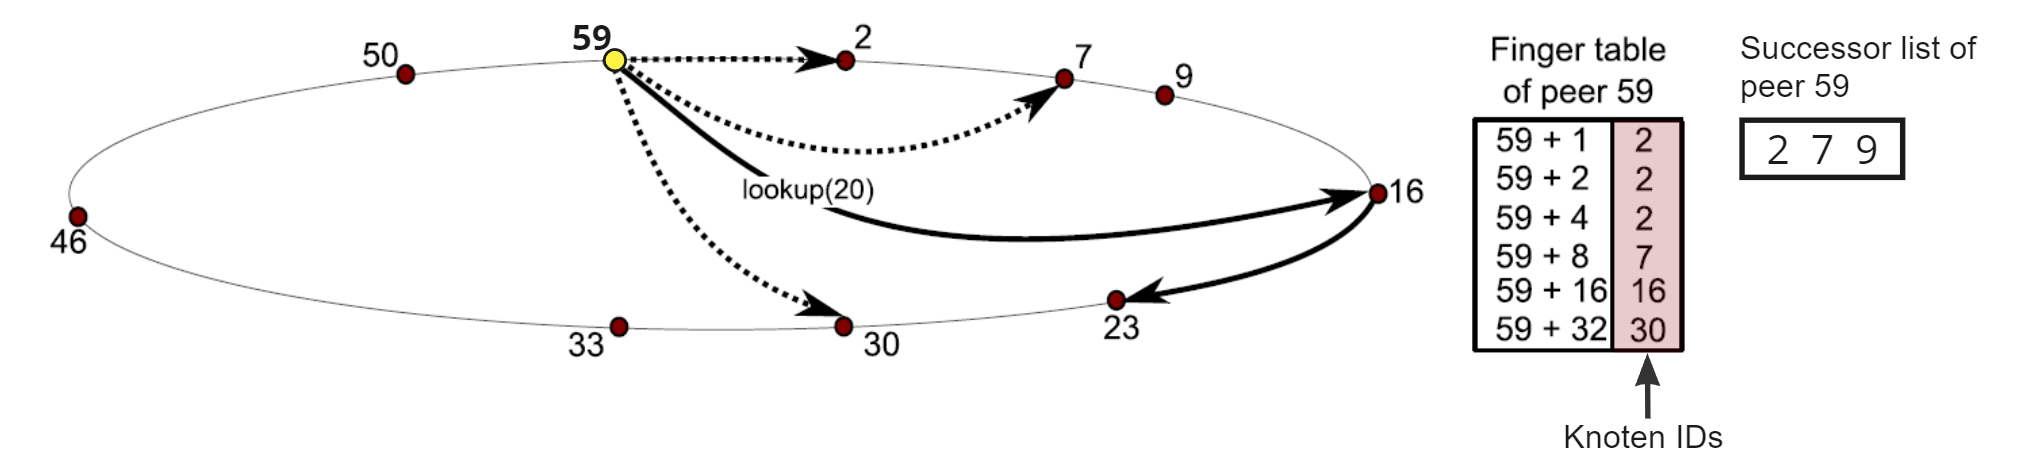
\includegraphics[width=1\linewidth]{images/chord_ring_altered.png}
    \captionof{figure}{Visualisierung der Ringstruktur von Chord, in Anlehnung an \cite[S. 811]{MedranoChavez_ChordKademliaHighChurnScenarios}}
    \label{chord_ring}
\end{center}

\noindent Wenn das Chord-Netzwerk eine Suchanfrage erhält, gibt es zwei Strategien, um die Anfrage zu bearbeiten. In der ersten Strategie wird die Anfrage sequentiell von Knoten zu Knoten weitergeleitet, bis der Knoten gefunden wird, der für den Schlüsselbereich verantwortlich ist, in dem sich der gesuchte Schlüssel befindet. Für diese Suchstrategie ergibt sich daher eine Komplexität von $\mathcal{O}(n)$, wobei $n$ die Anzahl der Knoten im Netzwerk ist. Die zweite Strategie verwendet die Finger-Tabelle, um die Anzahl der Knoten zu reduzieren, die die Anfrage weiterleiten. Diese Strategie hat eine Komplexität von $\mathcal{O}(\log n)$, wobei $n$ die Anzahl der Knoten im Netzwerk ist \parencite[S. 810-811]{MedranoChavez_ChordKademliaHighChurnScenarios}. 

In Abbildung \ref{chord_ring} ist zu erkennen, dass Knoten $59$ eine Suchanfrage für den Knoten mit der ID $20$ beginnt. Unter Verwendung der Finger-Tabelle von Knoten $59$ wird die Anfrage an den Knoten gesendet, der am nächsten an Knoten $20$ liegt. In diesem Fall ist dies Knoten $16$. Knoten $16$ wiederum leitet die Anfrage an den Knoten weiter, der ebenfalls am nächsten an Knoten $20$ liegt, was Knoten $23$ ist. Knoten $23$ ist für den Schlüsselbereich verantwortlich, in dem sich der gesuchte Schlüssel befindet, und sendet daher die Antwort an Knoten $59$ zurück. Durch die Verwendung dieser Strategie wurde Knoten $20$ in nur zwei Schritten gefunden, anstatt in fünft Schritten, wenn die Anfrage sequentiell weitergeleitet worden wäre.    

\subsubsection{Kademlia}
Im Gegensatz dazu verwendet Kademlia eine K-Bucket-Struktur, die in Abbildung \ref{kademlia_tree} zu sehen ist, um eine effiziente Verwaltung von Knoteninformationen zu ermöglichen. Die K-Buckets enthalten eine Liste von Knoten für verschiedene Schlüsselbereiche basierend auf ihrer Nähe, die durch XOR-Distanzen der IDs berechnet wird. Die Verbindungen zwischen den Knoten sind asymmetrisch, und jeder Knoten speichert Informationen über andere Knoten in seinen K-Buckets. Bei der Suche nach einem bestimmten Schlüssel erfolgt das Routing durch die XOR-Entfernung, wodurch die nächsten Knoten für diesen Schlüssel gefunden werden.
% asymmetrisch -> Knoten A kann Knoten B kennen, aber Knoten B kennt Knoten A nicht

\begin{center}
    \captionsetup{type=figure}
    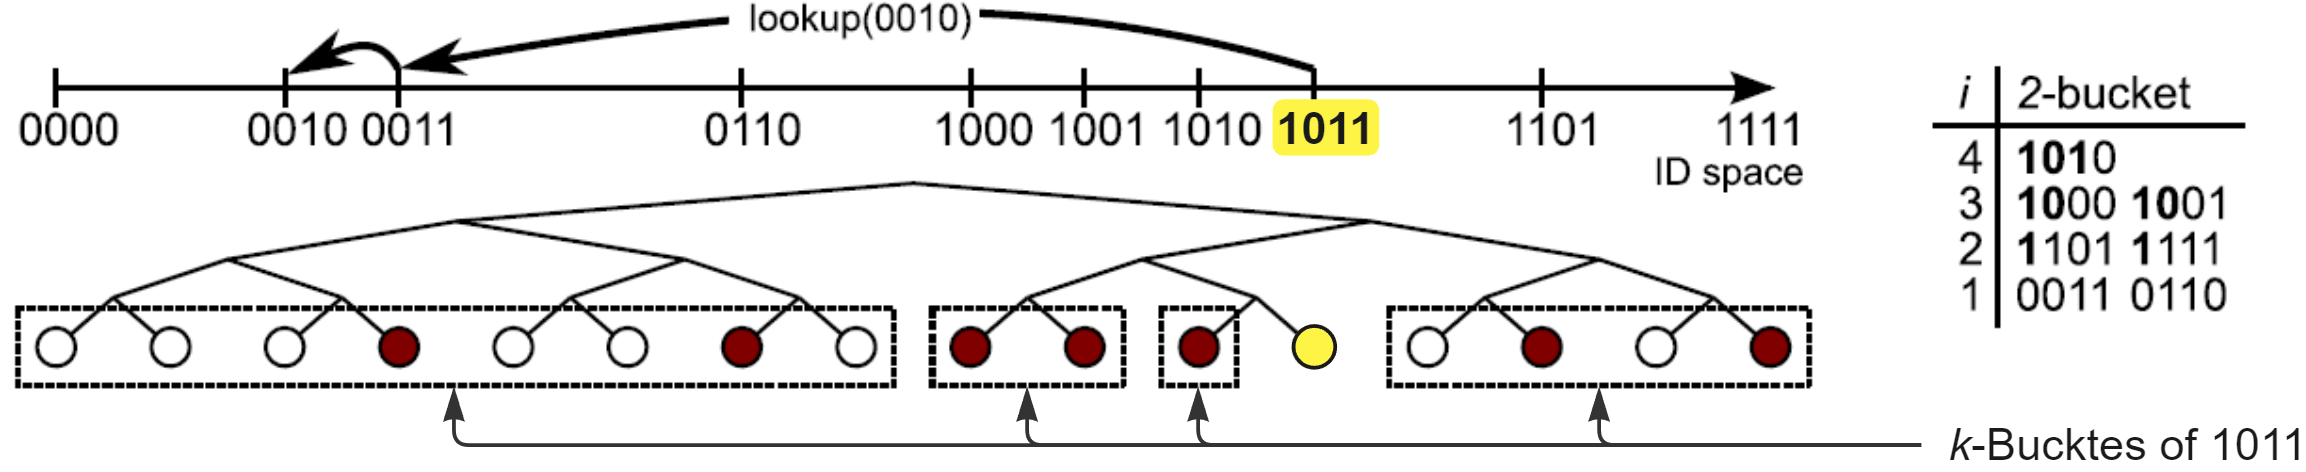
\includegraphics[width=1\linewidth]{images/kademlia_tree_altered.png}
    \captionof{figure}{Visualisierung der Baumstruktur von Kademlia, in Anlehnung an \cite[S. 812]{MedranoChavez_ChordKademliaHighChurnScenarios}}
    \label{kademlia_tree}
\end{center}

\noindent In Abbildung \ref{kademlia_tree} ist zu sehen, wie der Knoten $1011$ ein Suche nach Knoten $0010$ startet. Der Knoten $1011$ sucht in seinen vier K-Buckets nach dem nächsten Knoten, der am Schlüssel $0010$ liegt. Im ersten Bucket sind Knoten mit dem Präfix $0xxx$ enthalten. In Bucket zwei sind Knoten mit dem Präfix $11xx$, in Bucket drei Knoten mit dem Präfix $100x$ und in Bucket vier Knoten mit dem Präfix $101x$. Da der Schlüssel $0010$ mit dem Präfix $00$ beginnt, wird der nächste Knoten für diesen Schlüssel im ersten Bucket gesucht. Knoten $0011$ wird als nächster Knoten für den Schlüssel $0010$ gefunden. Knoten $1011$ sendet die Anfrage also an Knoten $0011$, der wiederum den nächsten Knoten für den Schlüssel $0010$ sucht. Da dieser Knoten den Schlüssel $0010$ in seinem K-Bucket besitzt, sendet er die Antwort auf die Suchanfrage an Knoten $1011$ zurück. Es werden zwei Weiterleitungen durchgeführt, um den Zielknoten zu finden, woraus sich eine Komplexität von $\mathcal{O}(\log n)$ ergibt, wobei $n$ die Anzahl der Knoten im Netzwerk ist \parencite[S. 812]{MedranoChavez_ChordKademliaHighChurnScenarios}.

Funktionen, wie diese Suche, werden durch die vier Nachrichten \textit{FIND\_NODE}, \\\textit{FIND\_VALUE}, \textit{PING} und \textit{STORE} des Kademlia-Protokolls ermöglicht. Sie haben die folgende Verwendung \Parencite[S. 3]{Maymounkov_Kademlia}:

\begin{itemize}
    \item \textit{FIND\_NODE}: Diese Nachricht wird verwendet, um den nächsten Knoten für einen bestimmten Schlüssel zu finden. Sie wird von einem Knoten an einen anderen Knoten gesendet, der den Schlüssel in seinem K-Bucket hat. Der Knoten, der die Nachricht erhält, antwortet mit einer Liste von Knoten, die den Schlüssel in ihrem K-Bucket haben \Parencite[S. 3]{Maymounkov_Kademlia}. 
    \item \textit{FIND\_VALUE}: Diese Nachricht wird verwendet, um den Wert für einen bestimmten Schlüssel zu finden. Sie wird von einem Knoten an einen anderen Knoten gesendet, der den Schlüssel in seinem K-Bucket hat. Der Knoten, der die Nachricht erhält, antwortet mit dem Wert, der dem Schlüssel zugeordnet ist, oder mit einer Liste von Knoten, die den Schlüssel in ihrem K-Bucket haben \Parencite[S. 3]{Maymounkov_Kademlia}.
    \item \textit{PING}: Diese Nachricht wird verwendet, um die Erreichbarkeit eines Knotens zu überprüfen. Sie wird von einem Knoten an einen anderen Knoten gesendet, um zu überprüfen, ob der Knoten noch erreichbar ist \Parencite[S. 2-3]{Maymounkov_Kademlia}.
    \item \textit{STORE}: Diese Nachricht wird verwendet, um einen Schlüssel-Wert-Paar in einem K-Bucket zu speichern. Sie wird von einem Knoten an einen anderen Knoten gesendet, um den Schlüssel-Wert-Paar in seinem K-Bucket zu speichern. Der Knoten, der die Nachricht erhält, speichert den Schlüssel-Wert-Paar in seinem K-Bucket \Parencite[S. 3]{Maymounkov_Kademlia}.
\end{itemize}

\noindent Da bei einem Instant-Messaging-Protokoll häufig Teilnehmer das Netzwerk verlassen und neue Teilnehmer dem Netzwerk beitreten, ist es wichtig, dass das Protokoll mit hoher Fluktuation umgehen kann. Diese Fluktuation von Nodes wird als Churn (engl. Abwanderung) bezeichnet. In einer Studie von Medrano-Chávez et al. \parencite{MedranoChavez_ChordKademliaHighChurnScenarios}, welche im hybriden Journal \textit{Peer-to-Peer Networking and Applications} veröffentlicht wurde, wurde die Leistung von Chord und Kademlia in Bezug auf Netzwerkfluktuation untersucht. Die Ergebnisse zeigen, dass Kademlia bei hoher Fluktuation besser abschneidet als Chord. Aus diesem Grund wird Kademlia in diesem Protokoll als Grundlage für das Auffinden von Teilnehmern und das Routing verwendet.

% #TODO: Warum Kademlia und was die Sicherheitsaspekte angeht, erst in Architektur aufgreifen.
    % Signaling Server könnte auch mit Anfragen geflutet werden -> der Sever könnte bei jedem checken, ob es sich um einen validen Teilnehmer handelt, was aber sehr aufwändig wäre
    % wenn Kademlia mit Anfragen geflutet wird, könnte es zu einem Denial of Service kommen, da die Knoten nicht mehr erreichbar sind -> habe aber ja mit dem Signaling Server noch eine weitere Instanz, die die Anfragen entgegen nimmt und weiterleitet

Durch die Entscheidung für die Implementierung von Kademlia als Grundlage für das Auffinden von Teilnehmern und das Routing, wird die Sicherheit des Protokolls beeinflusst. Da Kademlia ein dezentralisiertes Protokoll ist, ist es anfällig für den in Abschnitt \ref{subsubsec:sybil_attack} (\textit{\nameref{subsubsec:sybil_attack}}) beschriebenen Sybil-Angriff. Um diesen Angriff zu verhindern bzw. zu erschweren, wird in dieser Arbeit die Teilnahme am Netzwerk erst durch eine vorherige Registrierung ermöglicht. Die Registrierung wird durch die Blockchain-Technologie realisiert und ist mit Kosten verbunden, die ein Angreifer aufbringen muss, um am Netzwerk teilzunehmen. Da bei einem Sybil-Angriff der Angreifer mehrere Identitäten verwendet, um das Netzwerk zu übernehmen, muss er für jede Identität die Kosten aufbringen. Dadurch wird der Angriff erschwert, da der Angreifer mehr Ressourcen benötigt, um das Netzwerk zu übernehmen.







\begin{itemize}
    \item Kademlia vs. Angriffe
    \item Angriffe gegen ICE gucken und erklären
\end{itemize}

\noindent Sollte der Aufbau einer Direktverbindung mittels Kademlia nicht möglich sein, wird das Interactive Connectivity Establishment (ICE) Protokoll verwendet, um eine Verbindung zwischen zwei Teilnehmern herzustellen. ICE ist ein Framework, das mehrere Techniken kombiniert, um eine Verbindung zwischen zwei Endpunkten herzustellen, die sich hinter NATs befinden. Genaue Details zur Implementierung von ICE folgt in Kapitel \ref{subsec:verbindungsmanagement} \textit{\nameref{subsec:verbindungsmanagement}}.

\noindent Um die Problematik mit NATs zu lösen, wird das ICE-Protokoll verwendet. ICE ist ein Framework, das mehrere Techniken kombiniert, um eine Verbindung zwischen zwei Endpunkten herzustellen, die sich hinter NATs befinden. Genaue Details zur Implementierung von ICE folgt in Kapitel \ref{subsec:verbindungsmanagement} \textit{\nameref{subsec:verbindungsmanagement}}.


